\begin{figure*}[t]
	\centering
	\addtolength{\tabcolsep}{-4.5pt}
	\begin{tabular}{ccccccccc}
		Photo & Ours & \cite{Deschaintre2018} & \cite{Deschaintre2018}-Maps & & Photo & Ours & \cite{Deschaintre2018} & \cite{Deschaintre2018}-Maps
		\\
		\begin{overpic}[width=\resultwidth]{real/bump_1/target.jpg}
			\imglabel{Bump-3}
		\end{overpic} &
		\includegraphics[width=\resultwidth]{real/bump_1/good1.jpg} &
		
\includegraphics[width=\resultwidth]{egsr19/1_bump_real1/00.png} &
		\includegraphics[width=\resultwidth]{egsr19/1_bump_real1/tex2x2.jpg} &
		&
		\begin{overpic}[width=\resultwidth]{real/bump_2/target.jpg}
			\imglabel{Bump-4}
		\end{overpic} &
		\includegraphics[width=\resultwidth]{real/bump_2/good1.jpg} &
		
\includegraphics[width=\resultwidth]{egsr19/1_bump_real2/00.png} &
		\includegraphics[width=\resultwidth]{egsr19/1_bump_real2/tex2x2.jpg}
		\\
		\begin{overpic}[width=\resultwidth]{real/leather_1/target.jpg}
			\imglabel{Leather-3}
		\end{overpic} &
		\includegraphics[width=\resultwidth]{real/leather_1/good1.jpg} &
		
\includegraphics[width=\resultwidth]{egsr19/2_leather_real1/00.png} &
		\includegraphics[width=\resultwidth]{egsr19/2_leather_real1/tex2x2.jpg} &
		&
		\begin{overpic}[width=\resultwidth]{real/leather_2/target.jpg}
			\imglabel{Leather-4}
		\end{overpic} &
		\includegraphics[width=\resultwidth]{real/leather_2/good1.jpg} &
		
\includegraphics[width=\resultwidth]{egsr19/2_leather_real2/00.png} &
		\includegraphics[width=\resultwidth]{egsr19/2_leather_real2/tex2x2.jpg}
		\\
		\begin{overpic}[width=\resultwidth]{real/leather_3/target.jpg}
			\imglabel{Leather-5}
		\end{overpic} &
		\includegraphics[width=\resultwidth]{real/leather_3/good1.jpg} &
		
\includegraphics[width=\resultwidth]{egsr19/2_leather_real3/00.png} &
		\includegraphics[width=\resultwidth]{egsr19/2_leather_real3/tex2x2.jpg} &
		&
		\begin{overpic}[width=\resultwidth]{real/leather_4/target.jpg}
			\imglabel{Leather-6}
		\end{overpic} &
		\includegraphics[width=\resultwidth]{real/leather_4/good1.jpg} &
		
\includegraphics[width=\resultwidth]{egsr19/2_leather_real4/00.png} &
		\includegraphics[width=\resultwidth]{egsr19/2_leather_real4/tex2x2.jpg}
		\\
		\begin{overpic}[width=\resultwidth]{real/plaster_1/target.jpg}
			\imglabel{Plaster-3}
		\end{overpic} &
		\includegraphics[width=\resultwidth]{real/plaster_1/good1.jpg} &
		
\includegraphics[width=\resultwidth]{egsr19/3_plaster_real1/00.png} &
		\includegraphics[width=\resultwidth]{egsr19/3_plaster_real1/tex2x2.jpg} &
		&
		\begin{overpic}[width=\resultwidth]{real/plaster_2/target.jpg}
			\imglabel{Plaster-4}
		\end{overpic} &
		\includegraphics[width=\resultwidth]{real/plaster_2/good1.jpg} &
		
\includegraphics[width=\resultwidth]{egsr19/3_plaster_real2/00.png} &
		\includegraphics[width=\resultwidth]{egsr19/3_plaster_real2/tex2x2.jpg}
		\\
		\begin{overpic}[width=\resultwidth]{real/flake_1/target.jpg}
			\imglabel{Metallicflake-3}
		\end{overpic} &
		\includegraphics[width=\resultwidth]{real/flake_1/good1.jpg} &
		
\includegraphics[width=\resultwidth]{egsr19/4_flake_real1/00.png} &
		\includegraphics[width=\resultwidth]{egsr19/4_flake_real1/tex2x2.jpg} &
		&
		\begin{overpic}[width=\resultwidth]{real/flake_2/target.jpg}
			\imglabel{Metallicflake-4}
		\end{overpic} &
		\includegraphics[width=\resultwidth]{real/flake_2/good1.jpg} &
		
\includegraphics[width=\resultwidth]{egsr19/4_flake_real2/00.png} &
		\includegraphics[width=\resultwidth]{egsr19/4_flake_real2/tex2x2.jpg}
		\\
		\begin{overpic}[width=\resultwidth]{real/metal_1/target.jpg}
			\imglabel{Brushmetal-3}
		\end{overpic} &
		\includegraphics[width=\resultwidth]{real/metal_1/good1.jpg} &
		
\includegraphics[width=\resultwidth]{egsr19/5_metal_real1/00.png} &
		\includegraphics[width=\resultwidth]{egsr19/5_metal_real1/tex2x2.jpg} &
		&
		\begin{overpic}[width=\resultwidth]{real/wood_1/target.jpg}
			\imglabel{Wood-3}
		\end{overpic} &
		\includegraphics[width=\resultwidth]{real/wood_1/good1.jpg} &
		
\includegraphics[width=\resultwidth]{egsr19/6_wood_real1/00.png} &
		\includegraphics[width=\resultwidth]{egsr19/6_wood_real1/tex2x2.jpg}
		\\
		\begin{overpic}[width=\resultwidth]{real/wood_2/target.jpg}
			\imglabel{Wood-4}
		\end{overpic} &
		\includegraphics[width=\resultwidth]{real/wood_2/good1.jpg} &
		
\includegraphics[width=\resultwidth]{egsr19/6_wood_real2/00.png} &
		\includegraphics[width=\resultwidth]{egsr19/6_wood_real2/tex2x2.jpg} &
		&
		\begin{overpic}[width=\resultwidth]{real/wood_3/target.jpg}
			\imglabel{Wood-5}
		\end{overpic} &
		\includegraphics[width=\resultwidth]{real/wood_3/good1.jpg} &
		
\includegraphics[width=\resultwidth]{egsr19/6_wood_real3/00.png} &
		\includegraphics[width=\resultwidth]{egsr19/6_wood_real3/tex2x2.jpg}
	\end{tabular}
	\captionsetup{labelfont=bf,textfont=it}
	\caption{\label{fig:Des}
		\textbf{Comparison} to the single input SVBRDF estimation method of Deschaintre et al. \cite{Deschaintre2018}. Due to the nature of the method, their texture patterns are closely aligned with the input image; however, the overall perceptual appearance match is usually worse than our method. In some cases, the method produces specular burn-in, as the strong highlight cannot be fully removed and causes holes in the resulting maps (Plaster-4, Metallicflake-4). Advanced BRDF models like brushed metal and metallic flakes are not explicitly handled by their method and usually fail.
	}
\end{figure*}